\subsection{Existing SysML Connection Diagram}\label{sec:sysml}

A SysML Internal Block Diagram in the context of INTO-CPS is referred to as a \emph{Connection Diagram}.
It is used to define the composition and connectivity of several FMUs. The connection diagram contains instances of FMUs (SysML Block instances) which are connected together by means of connectors to the input/output ports of the FMU instances. The connection diagram also enables association of existing FMUs to the block instances for a co-simulation.

\begin{figure}[bt]
\centering
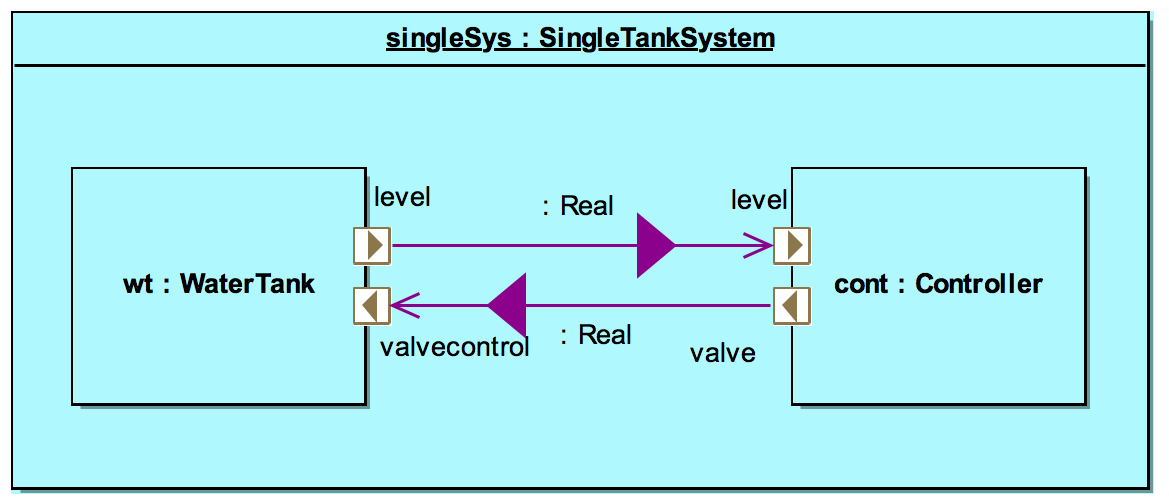
\includegraphics[width=.8\columnwidth]{Images/sysml_cd}
\caption{Connection diagram for the WaterTank example to connect FMUs.}
\label{fig:connection}
\end{figure}


Using a general-purpose modeling language such as SysML for defining simulation scenarios, comes with an inherent challenge.
The lack of simulation specific concepts in the language makes expression of these more cumbersome and error prone.
First, it is required that the users memorise the exact way these concepts must be expressed in SysML.
Secondly, it limits the assistance the tool can provide the user, due to its limited understanding of domain specific concepts.  
These issues are amplified by the fact that errors are only detected when the SysML model is imported in the tool.

In the DSE diagrams inside the SysML profile the exploration capabilities makes use of parameters for the different FMUs, so this is also important for the work we describe here.
